\documentclass[answers]{exam}
\usepackage{../../template}
\author{niceguy}
\title{Problem Set 2}
\begin{document}
\maketitle

\begin{questions}

\question{A line charge of finite length in free space has a density $Q' ( Q' > 0)$ along one its half and $-Q'$ along the other. The associated electric field intensity vector $\vec{E}$ at a point $M$ equally distant from the line ends is}

\begin{solution}
	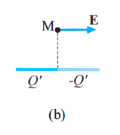
\includegraphics[width=0.3\textwidth]{1b.png}
\end{solution}

\question{Two parallel, infinite long strips of width $a$ are uniformly charged with equal charge densities $\rho_s(\rho_s>0)$, and a cross section of the structure is shown. The ambient medium is air, and the separation between strips is $d$. The resultant electric field intensity vector $\vec{E}$ at the point $M$ in the figure}

\begin{solution}
	has a negative $x$-component only
	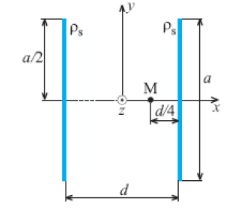
\includegraphics[width=0.3\textwidth]{2.png}
\end{solution}

\question{An infinitely long cylinder of radius $a$ in free space is charged with a volume charge density
	$$\rho_u = \rho_0\left(1-\frac{r}{a}\right)$$
	for $0\leq r\leq a$, where $\rho_0$ is a constant and $r$ is the radial coordinate in the cylindrical coordinate system. Find the charge per unit length on the cylinder.}

\begin{solution}
	\begin{align*}
		Q &= \int dQ \\
		  &= \iiint_V \rho_u dV \\
		  &= \int_0^L\int_0^{2\pi}\int_0^a \rho_0\left(1-\frac{r}{a}\right) rdr d\theta dz \\
		  &= 2\pi\rho_0L\left(\frac{a^2}{2}-\frac{a^2}{3}\right) \\
		\frac{Q}{L} &= \frac{2\pi\rho_0La^2}{3}
	\end{align*}
\end{solution}

\question{A cube of edge length $a$ in free space is charged with a volume charge density
	$$\rho_u = \rho_0\sin\left(\frac{\pi x}{a}\right), 0\leq x\leq a$$
wherer $\rho_0$ is a constant. Find the total charge in the cube.}

\begin{solution}
	\begin{align*}
		Q &= \iiint_V \rho_u dV \\
		  &= \int_0^a\int_0^a\int_0^a \rho_0\sin\left(\frac{\pi x}{a}\right)dxdydz \\
		  &= \rho_0a^2\times \frac{2a}{\pi} \\
		  &= \frac{2\rho_0a^3}{\pi}
	\end{align*}
\end{solution}

\question{Show that for large $z$, the electric field created on the $z$-axis (observation point $(0,0,z)$) by a semi-circular line charge with density $\rho_l$ at $z-0,r=a$ and $0\leq\phi <\pi$, is equivalent to the field of a point charge with the same amount of charge, located at the origin.}

\begin{solution}
	Using Cartesian Coordinates, the vector for $\vec{R}-\vec{R'}$ is
	$$-a\cos\phi\hat{i} - a\sin\phi\hat{j} + z\hat{k}$$
	Its magnitude is obviously
	$$\sqrt{a^2+z^2}$$
	Hence
	\begin{align*}
		\vec{E} &= k\int_0^\pi \frac{\rho_l(-a\cos\phi\hat{i} - a\sin\phi\hat{j} + z\hat{k})ad\phi}{(a^2+z^2)^{3/2}} \\
			&= k\frac{\rho_la}{(a^2+z^2)^{3/2}}(-2a\hat{j} + z\pi\hat{k}) \\
			&= k\frac{-2\rho_la^2}{(a^2+z^2)^{3/2}}\hat{j} + k\frac{\rho_laz\pi}{(a^2+z^2)^{3/2}}\hat{k}
	\end{align*}
	As $z\rightarrow\infty$, the first term goes to 0, and the second term goes to $k\frac{\rho_la\pi}{z^2}\hat{k}$. By inspection, the second term is equal to the field of a point charge with the same amount of charge located at the origin (total charge is equal to the numerator).
\end{solution}

\question{An infinite sheet of surface charge density $\rho_s$ on the $xy$-plane has a hole of radius $a$ on it, centered at the origin of the coordinate system. Find the electric field intensity at an arbitrary point on the positive $z$-axis.}

\begin{solution}
	Let that point be $(0,0,z)$. Then by symmetry, $\vec{E}$ is parallel to the $z$ axis. Then
	\begin{align*}
		E_z &= k\int_0^{2\pi}\int_a^\infty \frac{\rho_szrdrd\phi}{(r^2+z^2)^{3/2}} \\
			&= 2k\rho_sz\pi \int_{\arctan\left(\frac{a}{z}\right)}^{\frac{\pi}{2}} \frac{z^2\tan\theta\sec^2\theta d\theta}{z^3\sec^3\theta} \\
			&= 2k\rho_s\pi \int_{\arctan\left(\frac{a}{z}\right)}^{\frac{\pi}{2}} \sin\theta \\
			&= 2k\rho_s\pi \times \frac{z}{\sqrt{a^2+z^2}} \\
			&= \frac{2k\rho_s\pi z}{\sqrt{a^2+z^2}}
	\end{align*}
	Where the substitution $r=z\tan\theta$ is used.
\end{solution}

\question{For the structure composed of an infinitely long line charge distribution $\rho_l$ along the $z$-axis and a charged semi-cylinder with surface charge density $\rho_s$ at $r=a,0\leq\phi\leq\pi$, find the force per unit length on the semi-cylinder.} \label{this}

\begin{solution}
	$\vec{E}$ at any point on the cylinder is obviously parallel to $\hat{r}$ by symmetry.
	\begin{align*}
		E_r &= \int_{-\infty}^\infty \frac{k\rho_la}{(z^2+a^2)^{3/2}} dz \\
		    &= k\rho_la \int_{-\frac{\pi}{2}}^{\frac{\pi}{2}} \frac{a\sec^2\theta d\theta}{a^3\sec^3\theta} \\
		    &= k\rho_la \int_{-\frac{\pi}{2}}^{\frac{\pi}{2}} \frac{\cos\theta d\theta}{a^2} \\
		    &= \frac{2k\rho_l}{a}
	\end{align*}
	Where the substitution $z=a\tan\theta$ is used. \\
	By symmetry, net force is along the $y$-axis. Integrating for the force along this direction,
	\begin{align*}
		F_y &= \int_0^\pi\int_0^L \rho_s\sin\phi \times \frac{-2k\rho_l}{a^3} \times ad\phi dz \\
		\frac{F_y}{L} &= \frac{-2k\rho_l\rho_s}{a^2} \int_0^\pi \sin\phi d\phi \\
			      &= \frac{-4k\rho_l\rho_s}{a^2}
	\end{align*}
	So
	$$\vec{F} = -\frac{4k\rho_l\rho_s}{a^2}\hat{y}$$
\end{solution}

\question{Find the force between a charged circular loop of radius $b$ and uniform charge density $\rho_l$ and a point charge $Q$ located on the loop axis at a distance $h$ from the plane of the loop. What is the force when $h>>b$ and when $h=0$? Plot the force as a function of $h$.}

\begin{solution}
	By symmetry, the electric field at $Q$ is along the $z$ axis. Then
	\begin{align*}
		E_z &= \int_0^{2\pi} \frac{k\rho_lbhd\phi}{(b^2+h^2)^{3/2}} \\
		    &= \frac{2\pi k\rho_lbh}{(b^2+h^2)^{3/2}}
	\end{align*}
	The force is then
	$$\vec{F} = \frac{2\pi k\rho_lbhQ}{(b^2+h^2)^{3/2}}\hat{z}$$
	If $h>>b$, the denominator can be simplified to be $h^3$, so
	$$\vec{F} = \frac{2\pi k\rho_l bQ}{h^2}\hat{z}$$
\end{solution}

\question{A line charge of uniform density $\rho_l$ in free space forms a semicircle of radius $b$. Determine the magnitude and direction of the electric field intensity at the center of the semicircle.}

\begin{solution}
	We parametrize the line charge with $\phi\in[0,\pi]$, where by symmetry, the direction is along the $y$-axis. Then
	\begin{align*}
		E_y &= \int_0^\pi \frac{k\rho_lb\sin\phi d\phi}{b^2} \\
		    &= \frac{k\rho_l}{b} \times 2 \\
		    &= \frac{2k\rho_l}{b}
	\end{align*}
	So
	$$\vec{E} = -\frac{2k\rho_l}{b}\hat{y}$$
\end{solution}

\question{Three uniform line charges $\rho_{l1}, \rho_{l2}, \rho_{l3}$, each of length $L$, form an equilateral triangle. Assuming that $\rho_{l1} = 2\rho_{l2} = 2\rho_{l3}$, determine the electric field intensity at the center of the triangle.}

\begin{solution}
	Let $\rho_l = \rho_{l2} = \rho_{l3}$. Then let the first line charge $\rho_{l1}$ lie along the $x$-axis. If all line charges are the same, they will cancel out by symmetry. Hence by superposition, we can separately consider the contribution of the equilateral triangle with equal line charges, and the base with line charge $\rho_l$. The former cancels out to 0. For the latter, note that the height of the centre is $h = \frac{L}{2\sqrt{3}}$. Then
	\begin{align*}
		E_y &= \int_{-\frac{L}{2}}^{\frac{L}{2}} \frac{k\rho_lhdx}{(x^2+h^2)^{3/2}} \\
		    &= k\rho_lh \int_{-\frac{pi}{3}}^{\frac{\pi}{3}} \frac{h\sec^2\theta d\theta}{h^3\sec^3\theta} \\
		    &= k\rho_lh \int_{-\frac{pi}{3}}^{\frac{\pi}{3}} \frac{\cos\theta d\theta}{h^2} \\
		    &= \frac{\sqrt{3}k\rho_l}{h} \\
		    &= \frac{6k\rho_l}{L}
	\end{align*}
	Where the substitution $x=h\tan\theta$ is used.
\end{solution}

\question{For the structure composed of an infinitely long line charge distribution $\rho_l$ along the $z$-axis and a charged semi-cylinder with surface charge density $\rho_s$ at $r=a,\frac{\pi}{2}\leq\phi\leq\frac{3\pi}{2}$, find the force per unit length on the semi-cylinder.}

\begin{solution}
	Literally \ref{this} but rotated by $\frac{\pi}{2}$.
\end{solution}
\end{questions}
\end{document}
